
\subsection{Distribuované SŘBD}
Distribuovaný databázový systém (DDBS) je tvořen \textbf{distribuovanou bází dat} a \textbf{programovým vybavením}, skládajícím se z \textbf{lokálních SŘBD} a dalších programů potřebných k jejich \textbf{koordinaci a řízení}, k zabezpečení celosystémových úloh spojených s přístupem uživatelů k DDBS, s udržováním integrity a provozuschopnosti v prostředí počítačové sítě. \textbf{Uživateli se jeví celá distribuovaná báze jako by byla lokální} (na jednom místě) a přistupuje k ní stejným způsobem. 

Podle toho jak je dist. databáze řešena a kam směřují dotazy ji dělíme na: 

\subsubsection{Centralizované}
Mají popis a řízení DDBS soustředěno na \textbf{1 centrální počítač}. Toto centrum nemusí být v centru počítačové sítě. Jsou zde soustředěny \textbf{popisky všech dat} tvořících DDBS a \textbf{centrálně se řídí}: \textbf{přístup k datům}, \textbf{provádění změn} ve struktuře dat, \textbf{provádění a synchronizace transakcí} + všechny další činnosti systému. 
\begin{itemize}
	\item \textbf{Výhody} -- jedoduchost řízení.
	\item \textbf{Nevýhody} -- vysoké náklady na komunikaci, pomalost (každý přístup k datům musí být povolen centrem) a nebezpečí výpadku tohoto jednoho prvku.
\end{itemize}

\begin{figure}[H]
\centering
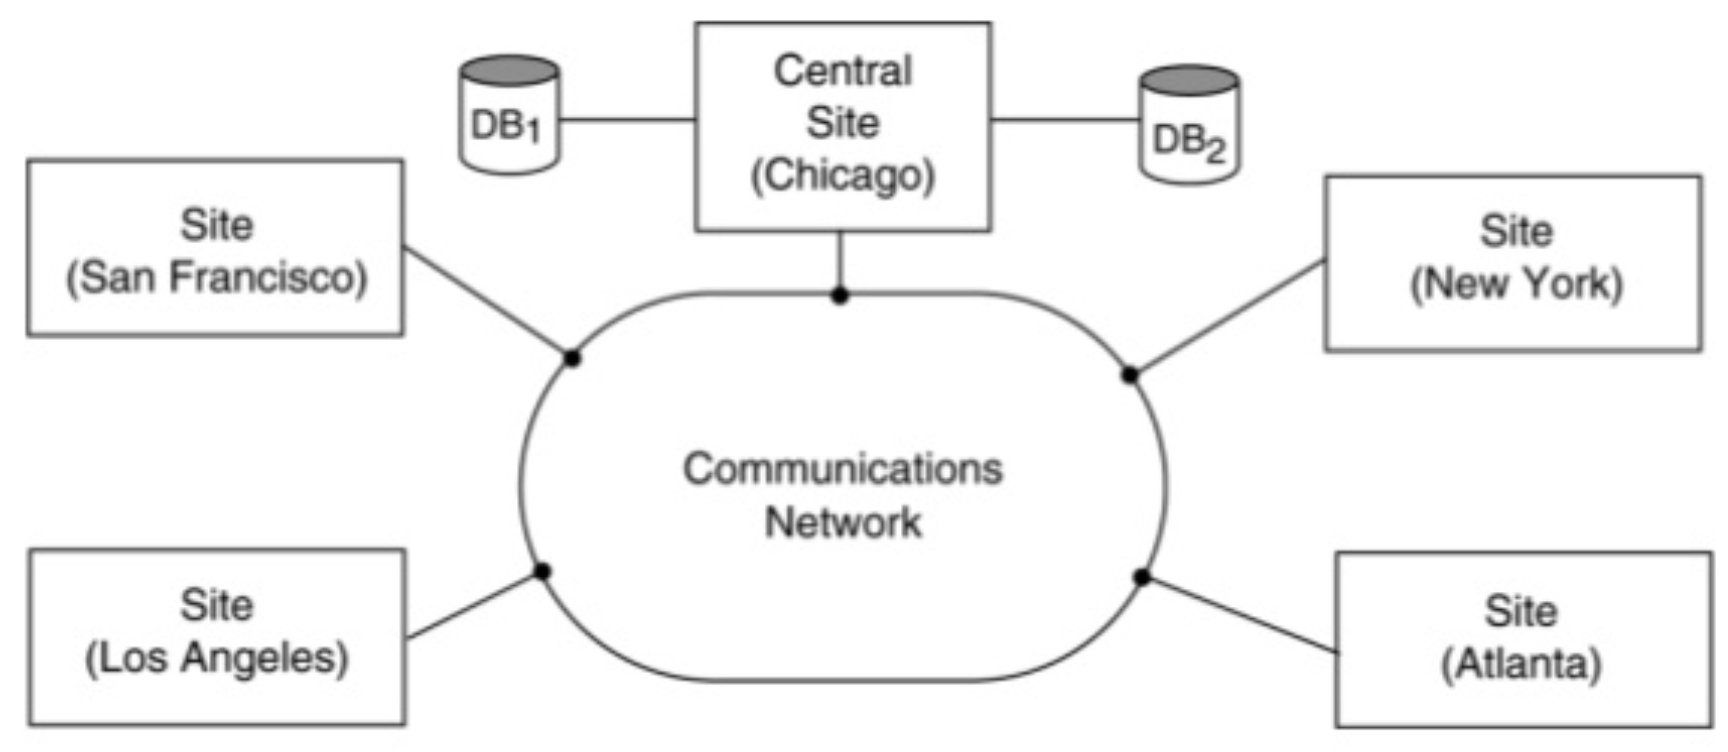
\includegraphics[width=0.8\textwidth]{assets/ddbs1.png}
\end{figure}

\subsubsection{Decentralizované}
Jsou tvořeny počítačovou sítí, kde žádný uzel nemá privilegované postavení. \textbf{Všechny počítače mají stejné informace o DDBS} a \textbf{stejnou odpovědnost za integritu DDBS}.
\begin{itemize}
	\item \textbf{Výhody} -- větší stabilita (výpadek počítače způsobí max. ztrátu přístupu k lokálním datům).
	\item \textbf{Nevýhody} -- složitější algoritmy pro řízení transakcí než v centralizovaných DDBS.
\end{itemize}

\begin{figure}[H]
\centering
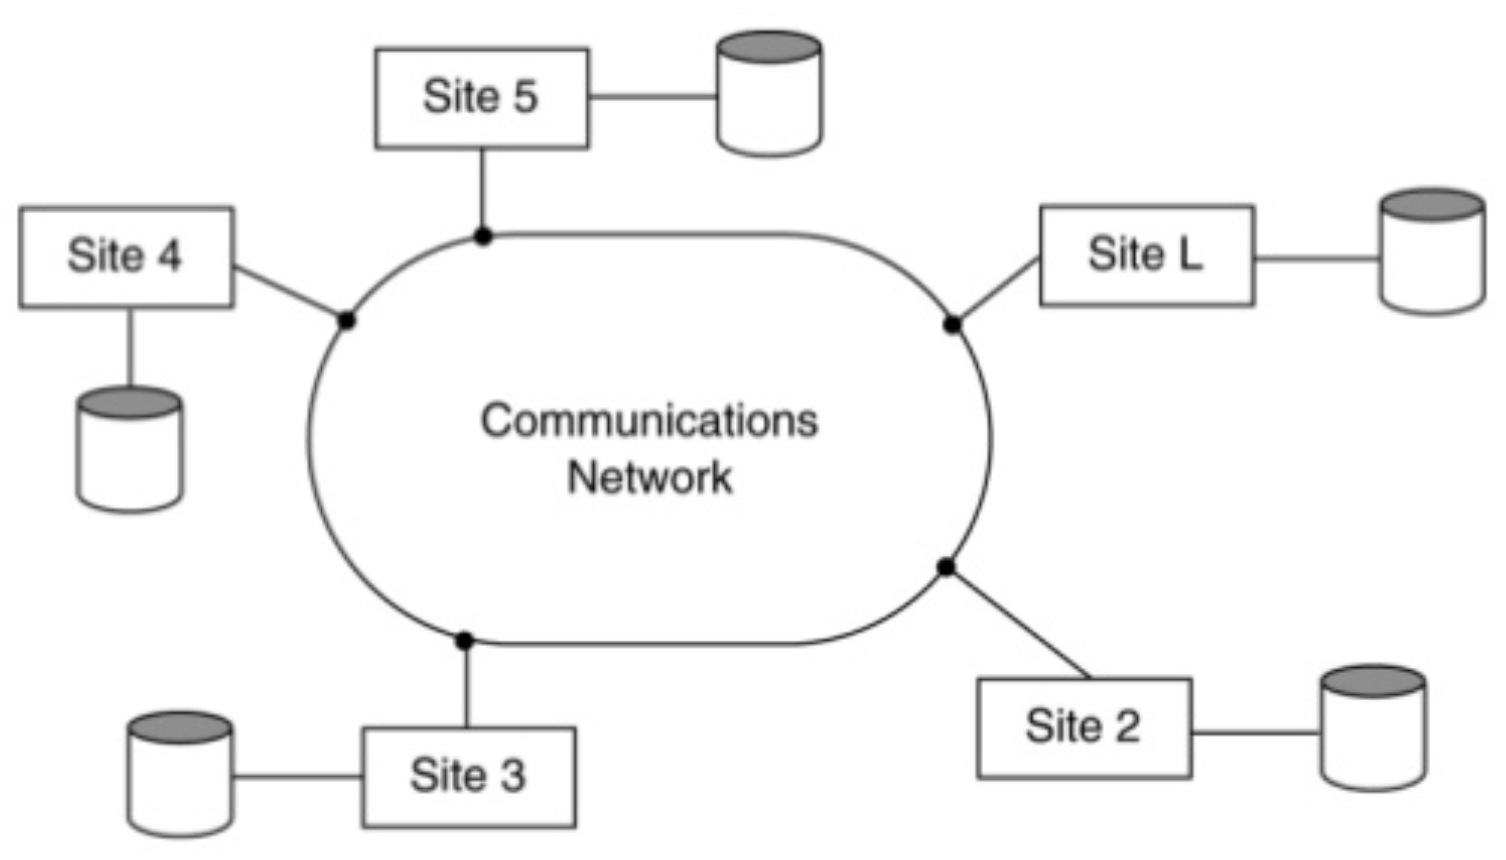
\includegraphics[width=0.8\textwidth]{assets/ddbs2.png}
\end{figure}

\subsection{Rozmístění dat (fragmentace a replikace)}
U DDBS jsou nejvíce časově náročné operace přesunu dat po komunikační lince. Vzhledem k vyšší možnosti poruch je třeba relace ukládat tak, aby jejich \textbf{dostupnost byla zajištěna} i v případě výpadku části sítě. Relací zde rozumíme logický celek, ale fyzicky i více souborů. Používají se \textbf{2 hlavní způsoby} fyzické implementace:
\begin{itemize}
	\item \textbf{Replikace} -- (přítomnost duplicitních dat) \textbf{uchovávání kopií relací v různých uzlech}, \textbf{porucha uzlu neznemožní přístup k relaci} (díky tomu se dist. databáze i samozálohuje), problém je v aktualizaci všech kopií relací. Proto se v DDBS ukládají v kopiích ta data, ke kterým je třeba \textbf{rychlý přístup} a nejsou často aktualizována a jsou velmi důležitá. 
	\item \textbf{Fragmentace} --  znamená \textbf{rozložení relací na menší části} (fragmenty), které jsou umístěny v různých
	uzlech sítě. Může jít o \textbf{horizontální} fragmentaci, kdy se v různých uzlech sítě ukládají části relace rozložené do skupin řádků nebo \textbf{vertikální} fragmentaci, kdy se v různých uzlech ukládají různé	projekce relací. Fragmentace se provádí, aby se \textbf{původní relace získala zpět standardními operacemi nad relační databází (sjednocení, spojení)}. 
\end{itemize}
Obě metody se často kombinují tak, že se v distribuované bázi uchovávají kopie fragmentů v různých uzlech.
V distribuované databázi musí být unikátní jména všech položek. Tedy ani 2 lokální položky nesmí používat
stejná jména pro různé položky. Jednou z možností jak tento problém vyřešit je \textbf{centrální slovník}, ovšem ten
je zase úzkým místem systému. 